\documentclass[a4paper,12pt,onecolumn,oneside]{article}
\usepackage{fontspec}
\usepackage[french]{babel}
\usepackage{minted}
\usepackage{graphicx}

\usepackage[margin=2.5cm]{geometry}
\usepackage{setspace}
\setlength{\parindent}{1cm}
\onehalfspacing
\hyphenation{}

\author{Alexandre Lionnet-Rollin \\ Master 1 HN \\ \texttt{https://github.com/Rollybre/rendu\_TAL}}
\title{Devoir pour la validation du séminaire de traitement automatique de la langue - Master HN}

\usepackage{hyperref}

\begin{document}
\maketitle
\bigskip

\section{Données}
Dans le cadre de la validation du séminaire de TAL, j'ai décidé d'appliquer les méthodes de \texttt{topic modeling} vues en cours. L'objectif est de caractériser les thèmes de mon corpus vis-à-vis de productions similaires.

\subsection{Rapide présentation du corpus}
Le corpus principal sur lequel j'ai travaillé est mon corpus de recherche dans le cadre de mon mémoire. Ce corpus est composé d'un genre de production littéraire nativement numérique appelé \emph{Creepypasta} : ce sont des courtes productions, la plupart du temps publiées sur des forums, à vocation horrifique, et dont le but, initialement, est d'être copiées puis collées. Analogues à la littérature fantastique par leur forme, ces histoires cherchent à flouter la limite entre la réalité et la fiction, en mettant en scène des narrateurs intradiégétiques et leur expérience virant souvent au cauchemar. Puisant à la fois dans le folklore et l'horreur, ces histoires se sont aujourd'hui sédimentées en un genre codifié.
Le corpus que j'ai construit compte près de vingt-trois mille histoires issues de deux plateformes distinctes : un fandom\footnote{\url{https://creepypasta.fandom.com/wiki/Creepypasta_Wiki}} et un subreddit\footnote{\url{https://www.reddit.com/r/nosleep/}} qui réunissent d'anciennes productions et de nouvelles qui sont ajoutées presque quotidiennement. 

Puisant dans l'esthétique traditionnelle de l'horreur, le but est de voir si cette appellation est justifiée et si les thèmes présents dans cette littérature recoupent les thèmes présents dans d'autres productions similaires en thèmes : les films d'horreur. 

En plus du corpus textuel, j'ai récupéré, à l'aide de l'API du site \emph{The Movie Database}, une liste de présentation de dix mille films d'horreur , s'étalant sur plus de cent ans. Ces présentations forment donc le second corpus auquel nous allons comparer les résultats.

\subsection{Choix de la méthode}
Afin de réaliser notre \emph{topic modeling}, plusieurs options s'offrent à nous. J'ai choisi d'utiliser BERTopic\footnote{\url{https://maartengr.github.io/BERTopic/index.html}} pour produire les thèmes, motivé par plusieurs raisons clés.

Tout d'abord, la modularité de BERTopic est un atout majeur, permettant de modifier facilement la méthode de vectorisation ou d'utiliser différents modèles, offrant ainsi une flexibilité précieuse pour la vérification empirique.

De plus, BERTopic est facile à utiliser et peu gourmand en ressources computationnelles. Par exemple, l'analyse de mon corpus avec BERTopic prend moins de 5 minutes et nécessite moins d'une dizaine de lignes de code, tandis qu'une LDA complète pour seulement la moitié de mon corpus prend plus de 5 heures.

BERTopic utilise BERT pour obtenir des représentations contextuelles des mots, offrant une modélisation des sujets plus précise et nuancée par rapport à LDA, qui ne prend pas en compte le contexte des mots.

Enfin, BERTopic propose des visualisations interactives des sujets, facilitant l'exploration et l'interprétation des résultats. LDA, bien que capable de produire des sujets interprétables, nécessite souvent des outils supplémentaires pour une visualisation équivalente.

\section{Prétraitement et présentation du code}
Le prétraitement des données est relativement sommaire : en effet, un autre des avantages de BERTopic réside dans l'ensemble des traitements effectués nativement, que ce soit la vectorisation, la tokenisation ou bien la production de plongements de mots.

J'ai néanmoins fait le choix de préciser la méthode de vectorisation (en l'occurrence tf-idf), qui permet d'ajouter une liste de stop-words à retirer. 
Pour notre corpus littéraire, j'ai utilisé une liste de stop-words personnalisée, produite à partir des mots les plus et les moins fréquents de mon corpus avec ajout progressif de mots au fur et à mesure des tentatives. 
Pour le corpus de présentation de films, j'ai utilisé la liste présente nativement dans la méthode de vectorisation TfIdf de sklearn.

Ainsi, voici le cœur du code utilisé pour le corpus de creepypastas \footnote{L'ensemble du notebook pourra être retrouvé sur le repo github associé} :

\begin{minted}{python}
vectorizer=TfidfVectorizer(stop_words=stop_words,ngram_range=(1,2))

topic_model = BERTopic(min_topic_size=35, 
                       verbose=True, 
                       vectorizer_model=vectorizer)
topics, _ = topic_model.fit_transform(liste_texte)

topic_model.visualize_barchart(top_n_topics=15,
                               n_words=10)
\end{minted}

On précise lors de la vectorisation l'étendue à étudier : j'ai choisi d'inclure les monogrammes et les bigrammes, combinaisons déjà suffisantes pour extraire les sujets (au-delà du bigramme, on perd rapidement en interprétabilité).

Une fois le modèle produit, nous utilisons une représentation en barres qui a le double avantage d'être visuelle tout en affichant les mots associés à chaque topic (au nombre de 10, afin d'avoir un aperçu suffisant de ce qui compose chaque topic).

\section{Résultats et comparaison}
Voici les 30 premiers topics obtenus :

\begin{figure}[htbp]
\centering
    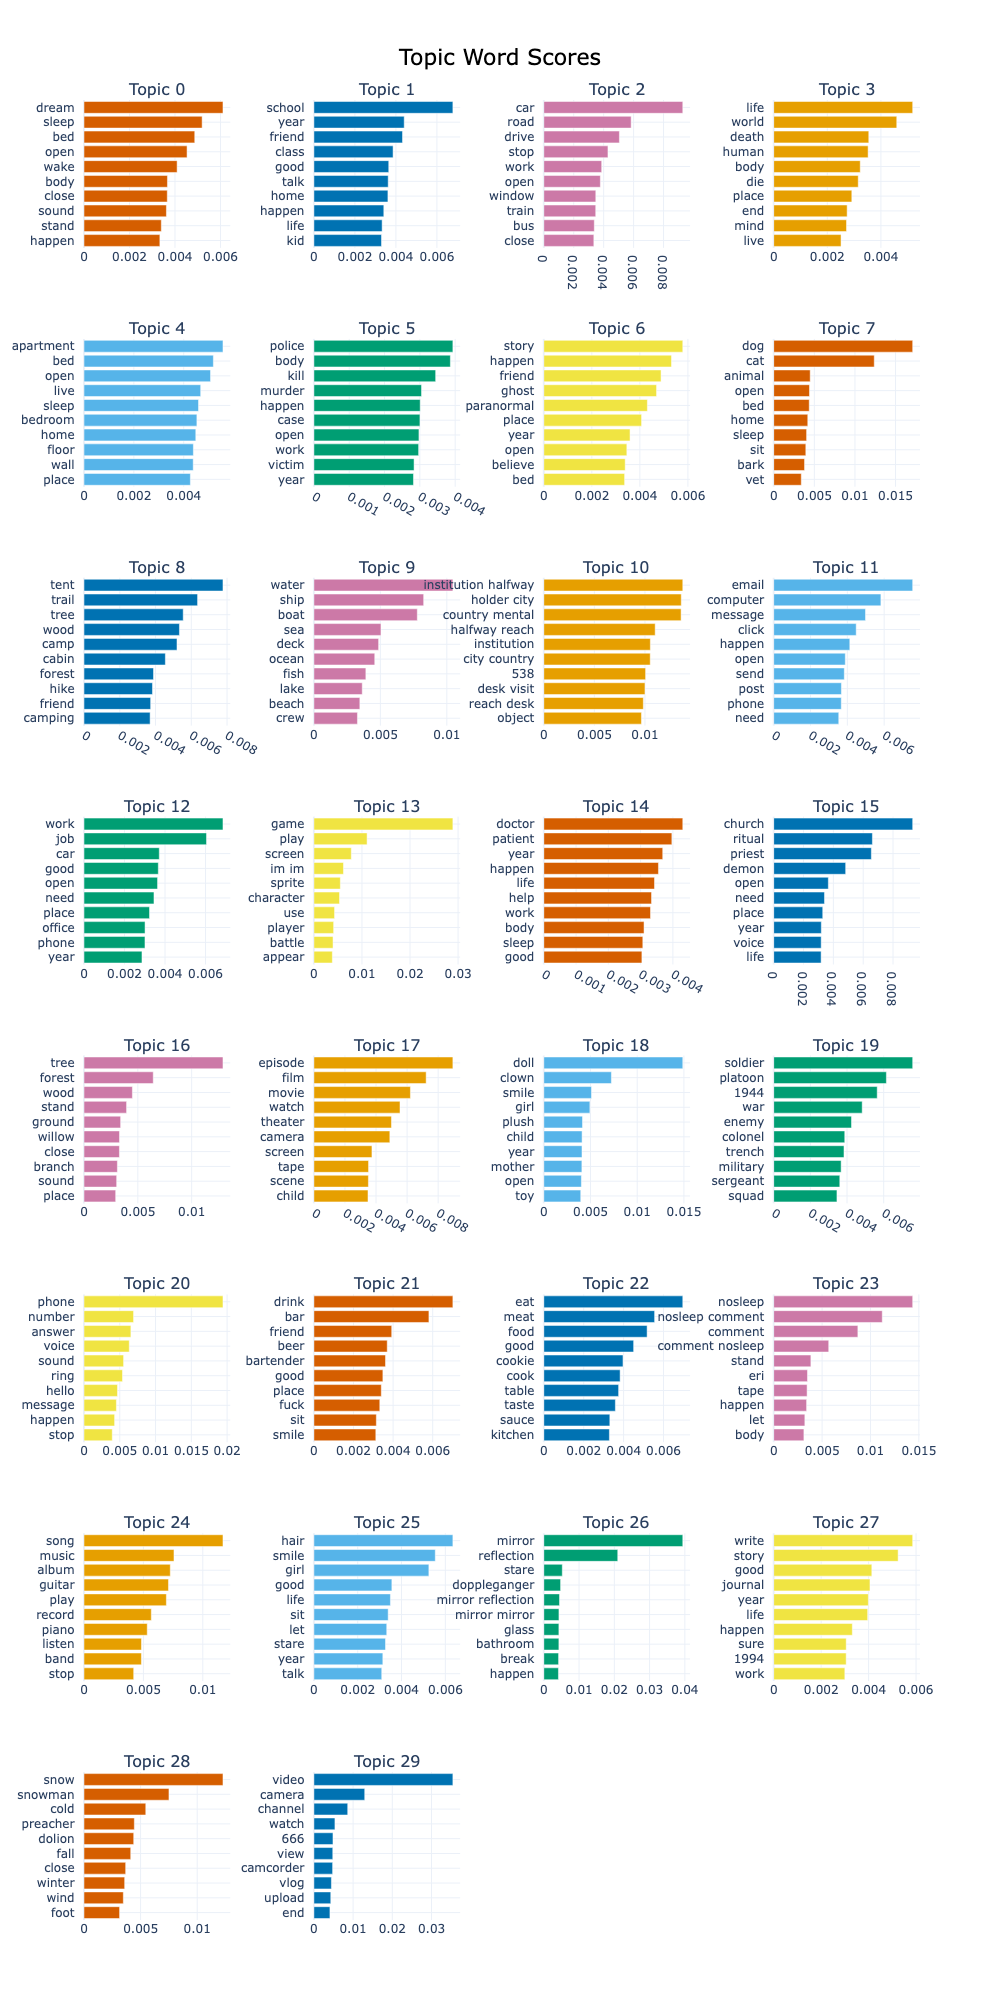
\includegraphics[scale=0.2]{bertopic_topic.png}
    \caption{Visualisation de 30 thèmes présents dans le corpus}
\end{figure}
\\

On note rapidement la présence des thèmes stéréotypiques de l'horreur : on retrouve les thèmes de la forêt et de l'isolation (topic 8 et topic 16), la vie ou la mort (topic 3), ou bien les thèmes de la religion (topic 15).

Néanmoins, certains thèmes semblent prévaloir, comme ceux de la technologie, et ce sous plusieurs formes (topic 11 : email, web ; topic 13 : jeux vidéo ; topic 17 : film/série ; topic 20 : téléphone ; topic 29 : vidéo). Ce thème semble plus surprenant, surtout dans sa multiplicité : la peur ici semble être liée à un aspect bien plus trivial, plus proche du quotidien.
Concernant le quotidien, la présence des thèmes comme celui de la nourriture, du sommeil, ou bien des relations amicales, nous amène à voir la notion de quotidien comme un élément caractéristique de ce genre.

\begin{figure}[htpb]
\centering
    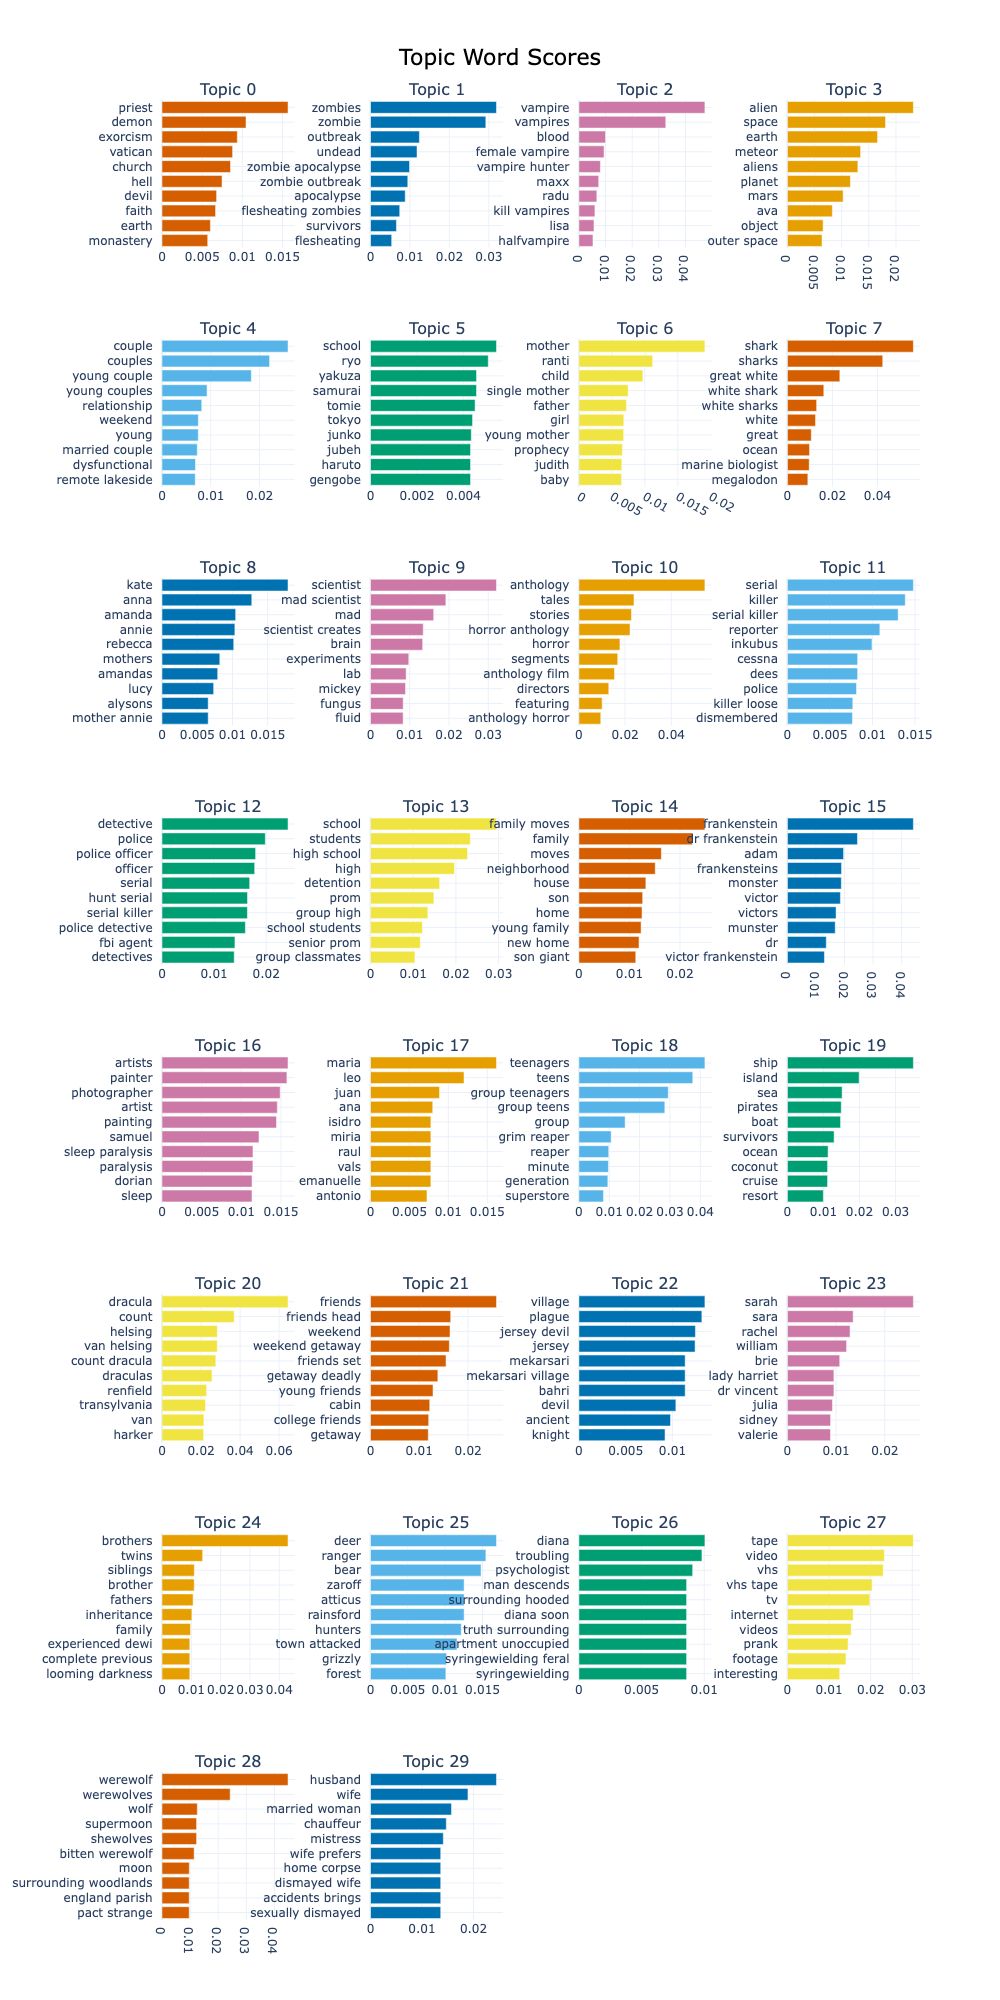
\includegraphics[scale=0.2]{bertopic_film.png}
    \caption{Visualisation de 30 thèmes présents dans les présentations de films}
\end{figure}

Concernant le corpus de présentation de films, qui nous sert ici de corpus de thème de référence pour le genre, on note dans un premier temps la présence marquée de thèmes plus spectaculaires et par la même stéréotypiques : les vampires, les zombies, le savant fou, les requins et les exorcismes sont présents, et forment des thèmes récurrents, présents dans notre imaginaire contemporain quand on parle d'horreur.

Si des thèmes sont présents dans les deux corpus (vie scolaire, amitié, famille), la question de leur valeur respective reste en suspens. Dans le cadre de l'horreur, les thèmes peuvent aussi bien être des éléments de cadre que des éléments qui sont à l'origine de la peur : les zombies sont des éléments à la fois terrifiants et cadrants, là où la famille peut être l'un ou l'autre ou les deux. On peut supposer, au vu de la fréquence des thèmes du quotidien dans le corpus littéraire, que ceux-ci sont dans la dernière catégorie : permettant à la fois de fixer le cadre, et, étant le cadre, permettent de produire le sentiment de peur une fois perverti.

\section{Conclusion}
Cette étude a montré que le \emph{topic modeling} avec BERTopic peut fournir des insights précieux sur les thèmes présents dans différents corpus textuels. En appliquant cette méthode à un corpus de creepypastas et à des descriptions de films d'horreur, nous avons pu identifier des thèmes récurrents et comparer les différences et similarités entre ces deux types de productions.

Les creepypastas, tout en partageant certains thèmes classiques de l'horreur avec les films, semblent se distinguer par une focalisation plus grande sur l'expérience personnelle et intime, souvent liée à la technologie et aux interactions quotidiennes. Cette différence pourrait être due à la nature plus personnelle et narrative des creepypastas par rapport aux descriptions plus stéréotypées et spectaculaires des films d'horreur.

Cependant, plusieurs limites doivent être prises en compte, notamment la dépendance aux représentations contextuelles de BERT, les défis posés par la diversité des corpus et la complexité des visualisations. La peur, si elle peut naître d'un thème, est souvent plus complexe et subtile : cette étude est une première étape, un dégrossissement qui vise à être approfondi plus tard.

\end{document}
